\documentclass[twocolumn,twoside,11pt,a4paper]{article}
\usepackage[utf8]{inputenc}     % 8 bits
\usepackage[pdftex]{graphicx}   % images .png or .pdf w/ pdflatex OR .eps w/ latex
\usepackage[T1]{fontenc}        % PS fonts
\usepackage{lmodern}            % fonts, sudo apt-get install lmodern
\usepackage{parskip}            % no indentation on paragraphs
\usepackage{tabularx}           % more on tables
\usepackage{longtable}          % more pages
\usepackage{url}                % URLs

\usepackage[sc]{mathpazo}       % Use the Palatino font
\linespread{1.05}               % Line spacing - Palatino needs more space between lines
\usepackage{microtype}          % Slightly tweak font spacing for aesthetics
\usepackage[hang, small, labelfont=bf,up,textfont=it,up]{caption} % Custom captions under/above floats in tables or figures
\usepackage{booktabs}           % Horizontal rules in tables
\usepackage{float}              % Required for tables and figures in the multi-column environment - they need to be placed in specific locations with the [H] (e.g. \begin{table}[H])
\usepackage{paralist}           % Used for the compactitem environment which makes bullet points with less space between them

% geometry package
\usepackage[outer=20mm,inner=20mm,vmargin=15mm,includehead,includefoot,headheight=15pt]{geometry}
%% space between columns
\columnsep 10mm

\usepackage{abstract}           % Allows abstract customization
\renewcommand{\abstractnamefont}{\normalfont\bfseries} % Set the "Abstract" text to bold
\renewcommand{\abstracttextfont}{\normalfont\small\itshape} % Set the abstract itself to small italic text

% \usepackage{titlesec}           % Allows customization of titles
% \renewcommand\thesection{\Roman{section}} % Roman numerals for the sections
% \renewcommand\thesubsection{\Roman{subsection}} % Roman numerals for subsections
% \titleformat{\section}[block]{\large\scshape\centering}{\thesection.}{1em}{} % Change the look of the section titles
% \titleformat{\subsection}[block]{\large}{\thesubsection.}{1em}{} % Change the look of the section titles

\usepackage[pdftex]{hyperref}
\hypersetup{%
    a4paper = true,              % use A4 paper 
    bookmarks = true,            % make bookmarks 
    colorlinks = true,           % false: boxed links; true: colored links
    pdffitwindow = false,        % page fit to window when opened
    pdfpagemode = UseNone,       % do not show bookmarks
    pdfpagelayout = SinglePage,  % displays a single page
    pdfpagetransition = Replace, % page transition
    linkcolor=blue,              % hyperlink colors
    urlcolor=blue,
    citecolor=blue,
    anchorcolor=green
}

\usepackage{indentfirst}         % indent also 1st paragraph

\usepackage{fancyhdr}            % Headers and footers
\pagestyle{fancy}                % pages have headers and footers
\fancyhead{}                     % Blank out the default header
\fancyfoot{}                     % Blank out the default footer
\fancyhead[LO,RE]{Exemplo de artigo em \LaTeX} % Custom header text
\fancyhead[RO,LE]{\thepage}      % Custom header text
\fancyfoot[RO,LE]{Grupo xx, \today} % Custom footer text
\renewcommand{\headrulewidth}{0.4pt}
\renewcommand{\footrulewidth}{0.4pt}

%\hyphenation{}                  % explicit hyphenation

%----------------------------------------------------------------------------------------
%	macro definitions
%----------------------------------------------------------------------------------------

% entities
\newcommand{\class}[1]{{\normalfont\slshape #1\/}}
\newcommand{\svg}{\class{SVG}}
\newcommand{\scada}{\class{SCADA}}
\newcommand{\scadadms}{\class{SCADA/DMS}}

%----------------------------------------------------------------------------------------
%	TITLE SECTION
%----------------------------------------------------------------------------------------

% article title
\title{\vspace{-15mm}\fontsize{24pt}{10pt}\selectfont\textbf{Spotify on the rocks}}

% authors
\author{Ana Santos\\
\small \texttt{ansantos3@gmail.com}\\
\and
Rui Pedro Lima\\
\small \texttt{ruipedro.lima@gmail.com}
\vspace{-5mm}
}

\date{\today}

%----------------------------------------------------------------------------------------

\begin{document}

\maketitle
\thispagestyle{plain}            % no headers in the first page

%----------------------------------------------------------------------------------------
%	ABSTRACT
%----------------------------------------------------------------------------------------

\begin{abstract}


Spotify on the Rocks é uma aplicação desenvolvida no âmbito da disciplina de Descrição,
Armazenamento e Processamento de Informação (DAPI), disciplina do 1º semestre do 5º ano
do Mestrado Integrado em Engenharia Informática e Computação (MIEIC) da Faculdade de
Engenharia da Universidade do Porto (FEUP).
A aplicação tem como principal objetivo obter grandes dimensões de informação musical,
interpretando-a ao nível do input do utilizador e representá-la de acordo com a sua
componente geográfica e métrica, oferecendo ao utilizador possíveis estudos e curiosidades
sobre os seus interesses musicais.

\end{abstract}

%----------------------------------------------------------------------------------------
%	ARTICLE CONTENTS
%----------------------------------------------------------------------------------------

\section{Introdução}\label{sec:intro}

%------------------------------------------------

Música faz parte do dia a dia de milhões de pessoas, seja através de dispositivos como
smartphones ou leitores de música portáteis, ou o habitual computador, sistema de hi-fi
ou até televisão, é indiscutível a importância e valor que esta arte tem.

%------------------------------------------------

\section{Contexto}\label{sec:application}

Spotify é, atualmente, a maior plataforma musical online e é famosa pela quantidade de
informação que possui sobre o negócio, mantendo além da informação sobre artistas, álbuns e
respetivas faixas, possui também imensa informação bastante precisa sobre os gêneros musicais,
origem geográfica e cronológica das obras e, limitado a quem possui uma conta (gratuita),
informação sobre o histórico de utilizadores bem como as preferências e construções dos
demais que constituem a comunidade virtual.
Toda a informação do Spotify está disponível sob forma de uma Application Programming Interface
(API) online, seguindo arquitetura REST (Representational State Transfer), oferecendo uma
colossal fonte de informação sobre artistas, álbuns, faixas e gêneros músicais, bem como a
recursos cronológicos sobre os trabalhos, informações geográficas dos artistas, estilos
associados e bandas relacionadas, bem como preferências e listas de reprodução construídas
pelos utilizadores.
A informação proveniente das pesquisas serão guardadas pela aplicação de forma a facilitar a
combinação com outros serviços, produzindo análises com teor analítico, facilitando o estudo
ou a descoberta de curiosidades fruto do cruzamento de dados.
A aplicação é responsável por recolher uma amostra de dados baseadas na informação
introduzida pelo utilizador ou, por omissão, descrever as últimas pesquisas efetuadas.
Embora a riqueza do serviço, apenas parte da API é usada para a aplicação.


%A arquitetura do visualizador assenta sobre os seguintes conceitos base \cite{kn:zpmd}:
%\begin{compactitem}
%\item \textbf{Componentes} --- Suspendisse auctor mattis augue \emph{push};
%\item \textbf{Praesent} --- Sit amet sem maecenas eleifend facilisis leo;
%\item \textbf{Pellentesque} --- Habitant morbi tristique senectus et netus.
%\end{compactitem}
%
%\begin{eqnarray}
%CIF_1: \hspace*{5mm}F_0^j(a) &=& \frac{1}{2\pi \iota} \oint_{\gamma} \frac{F_0^j(z)}{z - a} dz\\
%CIF_2: \hspace*{5mm}F_1^j(a) &=& \frac{1}{2\pi \iota} \oint_{\gamma} \frac{F_0^j(x)}{x - a} dx \label{eq:cif}
%\end{eqnarray}

%\subsection{Exemplo de Figura}

%É apresentado na Figura~\ref{fig:arch} %da página~\pageref{fig:arch}
%um exemplo de figura flutuante que ficará onde o \LaTeX\ entender.

%\begin{figure}
%  \begin{center}
%    \leavevmode
%    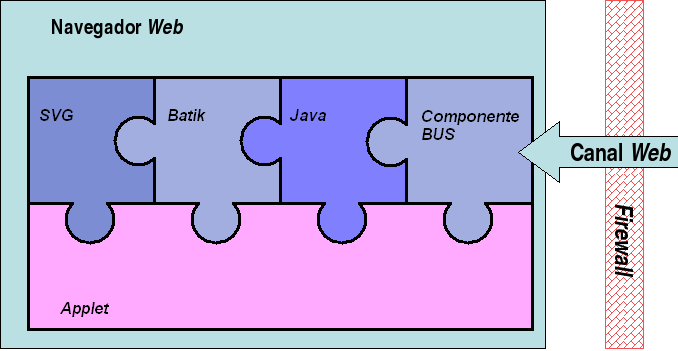
\includegraphics[width=0.45\textwidth]{puzzle}
%    \caption{Arquitetura da Solução Proposta}
%    \label{fig:arch}
%  \end{center}
%\end{figure}



% -----
% Exemplo de tableas
% -----
% \subsection{Exemplo de Tabela}

%É apresentado na Tabela~\ref{tab:exemplo1} um exemplo de tabela.

%\begin{table}[H]
%  \centering
%  \caption{Uma Tabela Simples}
%  \begin{tabular}{| l | p{45mm} |}
%    \hline
%    \textbf{Acrónimo} & \textbf{Significado}\\
%    \hline
%    \hline
%    ADT   & \emph{Abstract Data Type}\\\hline
%    ANDF  & \emph{Architecture-Neutral Distribution Format}\\\hline
%    API   & \emph{Application Programming Interface}\\
%    \hline
%  \end{tabular}
%  \label{tab:exemplo1}
%\end{table}

% \begin{table}
%   \centering
%   \caption{Tabela Exemplo}
% \begin{tabular}{|c|r@{.}lr@{.}lr@{.}l||r|}
% 	\hline
% \multicolumn{8}{|c|}
% 	{\rule[-3mm]{0mm}{8mm}Iteração $k$ de $f(x_n)$} \\
% \textbf{\em k}
% 	& \multicolumn{2}{c}{$x_1^k$}
% 	& \multicolumn{2}{c}{$x_2^k$}
% 	& \multicolumn{2}{c||}{$x_3^k$}
% 	& comentários \\ \hline \hline
% 0   & -0&3                 & 0&6                 &  0&7   & - \\
% 1   &  0&47102965 & 0&04883157 & -0&53345964  & $\delta<\epsilon$ \\
% 2   &  0&49988691 & 0&00228830 & -0&52246185  & $\delta < \varepsilon$ \\
% 3   &  0&49999976 & 0&00005380 & -0&523656   &   $N$ \\
% 4   &  0&5                 & 0&00000307 & -0&52359743  & \\
% \vdots	& \multicolumn{2}{c}{\vdots}
% 	& \multicolumn{2}{c}{$\ddots$}
% 	& \multicolumn{2}{c||}{\vdots}  & \\
% 7   &  0&5   & 0&0    & \textbf{-0}&\textbf{52359878}
% 		 & $\delta<10^{-8}$ \\ \hline
% \end{tabular}
%   \label{tab:exemplo2}
% \end{table}

%------------------------------------------------

\section{Conclusões}\label{sec:conclusions}

%----------------------------------------------------------------------------------------
%	REFERENCE LIST
%----------------------------------------------------------------------------------------

%% auto bibliographic list 
%\renewcommand{\bibname}{Referências}
% uses bibtex file
\bibliography{refs}
% format for PT/EN alpha/unsrt
%\bibliographystyle{alpha-pt}
%\bibliographystyle{alpha}
%\bibliographystyle{unsrt-pt}
%\bibliographystyle{unsrt}

%----------------------------------------------------------------------------------------

\end{document}
